\documentclass[11pt, a4paper]{article}
%

\usepackage{../caratuladc/caratula/caratula}

\usepackage{multicol}
\usepackage{enumitem}
\usepackage{xcolor}
\usepackage{etoolbox}

\newcommand{\hacer}{\textcolor{red}{HACER!}}
\newcommand{\punto}{\text{.}}
\usepackage[spanish,activeacute,es-tabla]{babel}
\usepackage[utf8]{inputenc}
\usepackage{ifthen}
\usepackage{listings}
\usepackage{dsfont}
\usepackage{subcaption}
\usepackage{amsmath}
\usepackage[top=1cm,bottom=2cm,left=1cm,right=1cm]{geometry}%
\usepackage{color}%
\usepackage{changepage}
\newcommand{\tocarEspacios}{%
	\addtolength{\leftskip}{3em}%
	\setlength{\parindent}{0em}%
}

\newcommand{\Indent}{\hspace*{0.75cm}}

% Especificacion de procs

\newcommand{\In}{\textsf{in }}
\newcommand{\Out}{\textsf{out }}
\newcommand{\Inout}{\textsf{inout }}

\newcommand{\encabezadoDeProc}[4]{%
% Ponemos la palabrita problema en tt
%  \noindent%
{\normalfont\bfseries\ttfamily proc}%
% Ponemos el nombre del problema
\ %
{\normalfont\ttfamily #2}%
\
% Ponemos los parametros
(#3)%
\ifblank{#4}{}{%
	% Por ultimo, va el tipo del resultado
	\ : #4}
}

\newenvironment{proc}[4][res]{%

% El parametro 1 (opcional) es el nombre del resultado
% El parametro 2 es el nombre del problema
% El parametro 3 son los parametros
% El parametro 4 es el tipo del resultado
% Preambulo del ambiente problema
% Tenemos que definir los comandos requiere, asegura, modifica y aux
\newcommand{\requiere}[2][]{%
{\normalfont\bfseries\ttfamily requiere\;}%
\ifthenelse{\equal{##1}{variaslineas}}{\{%
\begin{adjustwidth}{+5em}{}
	\ensuremath{##2}
\end{adjustwidth}
\}
{\normalfont\bfseries\,\par}%
}
{%
\{\ensuremath{##2}\}%
{\normalfont\bfseries\,\par}%
}
}

\newcommand{\asegura}[2][]{%
{\normalfont\bfseries\ttfamily asegura\;}%
\ifthenelse{\equal{##1}{variaslineas}}{\{%
\begin{adjustwidth}{+5em}{}
	\ensuremath{##2}
\end{adjustwidth}
\}
{\normalfont\bfseries\,\par}%
}
{%
\{\ensuremath{##2}\}%
{\normalfont\bfseries\,\par}%
}
}
\renewcommand{\aux}[4]{%
	{\normalfont\bfseries\ttfamily aux\ }%
		{\normalfont\ttfamily ##1}%
	\ifthenelse{\equal{##2}{}}{}{\ (##2)}\ : ##3\, = \ensuremath{##4}%
	{\normalfont\bfseries\,;\par}%
}
\renewcommand{\pred}[3]{%
{\normalfont\bfseries\ttfamily pred }%
	{\normalfont\ttfamily ##1}%
\ifthenelse{\equal{##2}{}}{}{\ (##2) }%
\{%
\begin{adjustwidth}{+5em}{}
	\ensuremath{##3}
\end{adjustwidth}
\}%
{\normalfont\bfseries\,\par}%
}

\newcommand{\res}{#1}
\vspace{1ex}
\noindent
\encabezadoDeProc{#1}{#2}{#3}{#4}
% Abrimos la llave
\par%
\tocarEspacios
}
{
% Cerramos la llave
\vspace{1ex}
}

\newcommand{\aux}[4]{%
	{\normalfont\bfseries\ttfamily\noindent aux\ }%
		{\normalfont\ttfamily #1}%
	\ifthenelse{\equal{#2}{}}{}{\ (#2)}\ : #3\, = \ensuremath{#4}%
	{\normalfont\bfseries\,;\par}%
}

\newcommand{\pred}[3]{%
{\normalfont\bfseries\ttfamily\noindent pred }%
	{\normalfont\ttfamily #1}%
\ifthenelse{\equal{#2}{}}{}{\ (#2) }%
\{%
\begin{adjustwidth}{+2em}{}
	\ensuremath{#3}
\end{adjustwidth}
\}%
{\normalfont\bfseries\,\par}%
}

% Tipos

\newcommand{\nat}{\ensuremath{\mathbb{N}}}
\newcommand{\reals}{\ensuremath{\mathbb{R}}}
\newcommand{\ent}{\ensuremath{\mathds{Z}}}
\newcommand{\float}{\ensuremath{\mathds{R}}}
\newcommand{\bool}{\ensuremath{\mathsf{Bool}}}
\newcommand{\cha}{\ensuremath{\mathsf{Char}}}
\newcommand{\str}{\ensuremath{\mathsf{String}}}
\newcommand{\dict}[1]{\ensuremath{\mathsf{dict}\lrangle{#1}}}
\newcommand{\conj}[1]{\ensuremath{\mathsf{conj}\lrangle{#1}}}
\newcommand{\tupla}[1]{\ensuremath{\mathsf{tupla}\lrangle{#1}}}
\newcommand{\struct}[1]{\ensuremath{\mathsf{struct}\lrangle{#1}}}

% Logica

\newcommand{\True}{\ensuremath{\mathrm{true}}}
\newcommand{\False}{\ensuremath{\mathrm{false}}}
\newcommand{\Then}{\ensuremath{\rightarrow}}
\newcommand{\Iff}{\ensuremath{\leftrightarrow}}
\newcommand{\implica}{\ensuremath{\longrightarrow}}
\newcommand{\IfThenElse}[3]{\ensuremath{\mathsf{if}\ #1\ \mathsf{then}\ #2\ \mathsf{else}\ #3\ \mathsf{fi}}}
\newcommand{\If}[3]{\text{\normalfont\ttfamily IfThenElse}(\ensuremath{#1,\;#2,\;#3})}
\newcommand{\yLuego}{\land _L}
\newcommand{\oLuego}{\lor _L}
\newcommand{\thenLuego}{\Then _L}

\newcommand{\cuantificador}[5]{%
	\ensuremath{(#2 #3: #4)\ (%
		\ifthenelse{\equal{#1}{multLineas}}{
			$ % exiting math mode
				\begin{adjustwidth}{+2em}{}
					$#5$%
				\end{adjustwidth}%
			$ % entering math mode
		}{
			#5
		}
		)}
}

\newcommand{\existe}[4][]{%
	\cuantificador{#1}{\exists}{#2}{#3}{#4}
}
\newcommand{\paraTodo}[4][]{%
	\cuantificador{#1}{\forall}{#2}{#3}{#4}
}

\newcommand{\Def}[1]{\text{\normalfont\ttfamily def}(#1)}

%listas

\newcommand{\TLista}[1]{\ensuremath{seq \langle #1\rangle}}
\newcommand{\lvacia}{\ensuremath{\langle\,\rangle}}
\newcommand{\lv}{\ensuremath{\langle\,\rangle}}
\newcommand{\longitud}[1]{\ensuremath{|#1|}}
\newcommand{\cons}[1]{\ensuremath{\mathsf{addFirst}}(#1)}
\newcommand{\indice}[1]{\ensuremath{\mathsf{indice}}(#1)}
\newcommand{\conc}[1]{\ensuremath{\mathsf{concat}}(#1)}
\newcommand{\head}[1]{\ensuremath{\mathsf{head}}(#1)}
\newcommand{\tail}[1]{\ensuremath{\mathsf{tail}}(#1)}
\newcommand{\sub}[1]{\ensuremath{\mathsf{subseq}}(#1)}
\newcommand{\en}[1]{\ensuremath{\mathsf{en}}(#1)}
\newcommand{\cuenta}[2]{\mathsf{cuenta}\ensuremath{(#1, #2)}}
\newcommand{\suma}[1]{\mathsf{suma}(#1)}
\newcommand{\twodots}{\ensuremath{\mathrm{..}}}
\newcommand{\masmas}{\ensuremath{+\!+\;}}
\newcommand{\matriz}[1]{\TLista{\TLista{#1}}}
\newcommand{\seqchar}{\TLista{\cha}}
\newcommand{\lrangle}[1]{\ensuremath{\langle#1\rangle}}

%dict

\newcommand{\setKey}[1]{\ensuremath{\mathsf{setKey}(#1)}}
\newcommand{\delKey}[1]{\ensuremath{\mathsf{delKey}(#1)}}

\renewcommand{\wp}[2]{
	\ensuremath{\textit{wp}(\textbf{\lstinline{#1}}, #2)}
}

\newcommand{\hoare}[3]{\ensuremath{\{#1\} \; #2 \; \{#3\}}}

\renewcommand{\lstlistingname}{Código}
\lstset{% general command to set parameter(s)
	language=Java,
	morekeywords={func, endif, endwhile, skip, end, var, then},
	basewidth={0.47em,0.40em},
	columns=fixed, fontadjust, resetmargins, xrightmargin=5pt, xleftmargin=15pt,
	flexiblecolumns=false, tabsize=4, breaklines, breakatwhitespace=false, extendedchars=true,
	numbers=left, numberstyle=\tiny, stepnumber=1, numbersep=9pt,
	frame=l, framesep=3pt,
	captionpos=b,
}

% TADs

\newenvironment{tad}[2]{
\newcommand{\tadtype}{%
	\ensuremath{#1 \ifblank{#2}{}{\lrangle{#2}}}
}

\renewcommand{\pred}[3]{%
{\normalfont\bfseries\ttfamily pred }%
	{\normalfont\ttfamily ##1}%
\ifthenelse{\equal{##2}{}}{}{\ (##2) }%
\{%
\begin{adjustwidth}{+5em}{}
	\ensuremath{##3}
\end{adjustwidth}
\}
{\normalfont\bfseries\,\par}%
}

\vspace{1ex}
\noindent
{\normalfont\bfseries\ttfamily\large TAD #1\ifthenelse{\equal{#2}{}}{}{$<$#2$>$}} \{
% Abrimos la llave
\par%
\tocarEspacios
}{
\vspace{1ex} \par\}
}

\newcommand{\obs}[2]{
	obs #1: \ensuremath{#2}\par
}

\newenvironment{module}[4]{
\newcommand{\tadtype}{%
	\ensuremath{#3 \ifblank{#4}{}{\lrangle{#4}}}
}

\newcommand{\moduletype}{%
	\ensuremath{#1 \ifblank{#2}{}{\lrangle{#2}}}
}


\renewcommand{\pred}[3]{%
{\normalfont\bfseries\ttfamily pred }%
	{\normalfont\ttfamily ##1}%
\ifthenelse{\equal{##2}{}}{}{\ (##2) }%
\{%
\begin{adjustwidth}{+5em}{}
	\ensuremath{##3}
\end{adjustwidth}
\}
{\normalfont\bfseries\,\par}%
}

\vspace{1ex}
\noindent
{\normalfont\bfseries\ttfamily\large Módulo #1\ifthenelse{\equal{#2}{}}{}{$<$#2$>$} implementa #3\ifthenelse{\equal{#4}{}}{}{$<$#4$>$}} \{
% Abrimos la llave
\par%
\tocarEspacios
}{
\vspace{1ex} \par\}
}

\newcommand{\var}[2]{
	var #1: \;\ensuremath{#2}\par
}
\newcommand{\compl}[1]{Complejidad: $#1$}

% Tipos de datos de implementación
\newcommand{\Int}{\ensuremath{\mathsf{int}}}
\newcommand{\Real}{\ensuremath{\mathsf{real}}}
\newcommand{\Bool}{\ensuremath{\mathsf{bool}}}
\newcommand{\Char}{\ensuremath{\mathsf{char}}}
\newcommand{\String}{\ensuremath{\mathsf{string}}}
\newcommand{\Array}[1]{\ensuremath{\mathsf{Array<#1>}}}

\begin{document}

\titulo{Guia 6}
\materia{Algoritmos y Estructuras de Datos I}
\fecha{2do cuatrimestre 2024}

\integrante{Federico Barberón}{112/24}{jfedericobarberonj@gmail.com}
%Carátula
\maketitle
\newpage

%Indice
\tableofcontents
\newpage

\section{Guia 6}

\subsection{Ejercicio 1}
Implementamos el TAD Secuencia sobre una lista simplemente enlazada usando
\bigskip


NodoLista$<$T$>$ es struct$<$\par
\Indent valor: T,\par
\Indent siguiente: NodoLista$<$T$>$\par
$>$

\begin{module}{ListaEnlazada}{T}{Secuencia}{T}
	\newcommand{\node}{\text{NodoLista$<$T$>$}}
	\var{primero}{\node}
	\var{ultimo}{\node}
	\var{longitud}{\Int}

	\begin{proc}{NuevaListaVacía}{}{\moduletype}
		\begin{lstlisting}[numbers=none,frame=none]
		res := new ListaEnlazada< T >
		res.primero := null
		res.ultimo := null
		res.longitud := 0
		return res
		\end{lstlisting}
	\end{proc}

	\begin{proc}{AgregarAdelante}{\Inout l: \moduletype, \In e: T}{}
		\begin{lstlisting}[numbers=none,frame=none]
		nodo := new NodoLista< T >
		nodo.valor := e
		nodo.siguiente := null

		if l.longitud == 0 then
			l.primero := nodo
			l.ultimo := nodo
		else
			nodo.siguiente := l.primero
			l.primero := nodo
		endif
		l.longitud := l.longitud + 1
		\end{lstlisting}

	\end{proc}

	\begin{proc}{Pertenece}{\In l: \moduletype, \In e: T}{\Bool}
		\begin{lstlisting}[numbers=none,frame=none]
		res := false
		actual := l.primero
		while actual != null do
			if actual.valor == e then
				res := true
			endif
			actual := actual.siguiente
		endwhile
		return res
		\end{lstlisting}
	\end{proc}
\end{module}

\begin{itemize}
	\item Escriba los algoritmos para los siguientes procs y calcule su complejidad
	      \begin{itemize}
		      \item agregarAtras
		      \item obtener
		      \item eliminar
		      \item concatenar
	      \end{itemize}
	\item Escriba el invariante de representación para este módulo en castellano
	\item Dado el siguiente invrep, indiquie si es correcto. En caso de no serlo, corrijalo:

	      \pred{InvRep}{l: NodoLista$<$T$>$}{
		      accesible(l.primero,l.ultimo) \land largoOK(l.primero,l.longitud)
	      }

	      \pred{largoOK}{n: NodoLista$<$T$>$, largo: \ent}{
		      (n = null \land largo = 0) \lor (largoOK(n.siguiente, largo-1))
	      }

	      \pred{accesible}{$n_0$: NodoLista$<$T$>$, $n_1$: NodoLista$<$T$>$}{
		      n_1 = n_0 \lor (n_0.siguiente \neq null \yLuego accesible(n_0.siguiente, n_1))
	      }

\end{itemize}

{
\newcommand{\moduletype}{ListaEnlazada$<$T$>$}
\newcommand{\node}{\text{NodoLista$<$T$>$}}
\begin{proc}{agregarAtras}{\Inout l: \moduletype, \In e: T}{}
	\compl{O(1)}
	\begin{lstlisting}[numbers=none,frame=none]
	var nodo: NodoLista < T >;
	
	nodo := new NodoLista < T >;
	nodo.valor = e;

	if l.longitud == 0
		l.primero = nodo;
		l.ultimo = nodo;
	else
		l.ultimo.siguiente = nodo;
		l.ultimo = nodo;
	endif
	\end{lstlisting}
\end{proc}

\begin{proc}{obtener}{\In l: \moduletype, \In indice: \Int}{T}
	\compl{O(n)}
	\begin{lstlisting}[numbers=none,frame=none]
	var actual: NodoLista < T >
	var i: int;

	actual := l.primero;
	i := indice;

	while i > 0 do
		actual := actual.siguiente;
		i := i - 1;
	endwhile

	return actual.valor;
		\end{lstlisting}
\end{proc}

\begin{proc}{eliminar}{\Inout l: \moduletype, \In indice: \Int}{}
	\compl{O(n)}
	\begin{lstlisting}[numbers=none,frame=none]
	var actual: NodoLista < T >
	var i: int;
	
	actual := l.primero;
	i := indice;

	while i > 1 do
		actual := actual.siguiente;
		i := i - 1;
	endwhile

	actual.siguiente := actual.siguiente.siguiente;
	\end{lstlisting}
\end{proc}

\begin{proc}{concatenar}{\Inout l1: \moduletype, \In l2: \moduletype}{}
	\compl{O(m) \leftarrow m = Long(l2)}

	\begin{lstlisting}[numbers=none,frame=none]
	var actual: NodoLista < T >;
	var ultimo: NodoLista < T >;
	
	actual := l2.primero;
	ultimo := l1.ultimo;

	while actual != null do
		nodo := new NodoLista< T >
		nodo.valor = actual.valor;
		ultimo.siguiente = nodo;
		ultimo := nodo;
	endwhile
	\end{lstlisting}
\end{proc}

InvRep:
\begin{itemize}
	\item La lista no tiene ciclos
	\item La cantidad de nodos es igual a la longitud
	\item No existe nodo que apunte al primero, y el ultimo siempre apunta a null
	\item El primer nodo tiene una conexión indirecta con el último nodo
\end{itemize}

\pred{InvRep}{l: \moduletype}{
	accesible(l.primero,l.ultimo) \land largoOK(l.primero,l.longitud) \land \\
	sinCiclos(l.primero) \land l.ultimo.siguiente = null \land \\
	\paraTodo{n}{\node}{n.siguiente \neq l.primero}
}
}

\subsection{Ejercicio 2}
Implemente el TAD ConjuntoAcotado$<$T$>$ (definido en el apunte de TADs) usando la siguiente estructura.

\begin{module}{ConjuntoArr}{TAD}{ConjuntoAcotado}{T}
	\var{datos}{\Array{T}}
	\var{tamaño}{\Int}
\end{module}

\begin{itemize}
	\item Escriba el InvRep y la función Abs
	\item Escriba los algoritmos para las operaciones conjVacío y pertenece
	\item Escriba el algoritmo para la operación agregar
	\item Escriba los algoritmos para las operaciones unir e intersecar
	\item Escriba el algoritmo para la operación sacar.
	\item Calcule la complejidad de cada una de estas operaciones
	\item Qué cambios haría en su implementación si se quiere que la operación agregar sea lo más rápdia posible? Y si se quiere acelerar la operación buscar? Indique los cambios en la estructura, el InvRep, la función Abs y los algoritmos.
\end{itemize}

\pagebreak

\begin{module}{ConjuntoArr}{T}{ConjuntoAcotado}{T}
	\var{datos}{\Array{T}}
	\var{tamaño}{\Int}

	\pred{InvRep}{c: \moduletype}{
		c.tama\tilde{n}o \leq length(c.datos) \yLuego \paraTodo{i,j}{\ent}{0 \leq i < j < c.tama\tilde{n}o \thenLuego c.datos[i] \neq c.datos[j]}
	}


	\pred{predAbs}{c: \moduletype, c': \tadtype}{
		length(c.datos) = c'.capacidad \land \\
		\paraTodo{e}{T}{e \in c'.elems \iff \existe{i}{\Int}{0 \leq i < c.tama\tilde{n}o \yLuego c.datos[i] = e}}
	}

	\begin{proc}{conjVacío}{\In capacidad: \Int}{\moduletype}
		\compl{O(1)}
		\begin{lstlisting}[numbers=none,frame=none]
		var conj: ConjuntoArr < T >;

		conj := new ConjuntoArr < T >;
		conj.datos := new Array < T >[capacidad];
		conj.tamano := 0;
		return conj;
		\end{lstlisting}
	\end{proc}

	\begin{proc}{pertenece}{\In c: \moduletype, \In e: T}{\bool}
		\compl{O(n)}
		\begin{lstlisting}[numbers=none,frame=none]
		var i: int;
		i := 0;

		while i < c.tamano && c.datos[i] != e do
			i := i + 1;
		endwhile

		return i < c.tamano;
		\end{lstlisting}
	\end{proc}

	\begin{proc}{agregar}{\Inout c: \moduletype, \In e: T}{}
		\compl{O(n)}
		\begin{lstlisting}[numbers=none,frame=none]
		if !c.pertenece(e)
			c.datos[c.tamano] := e;
			c.tamano := c.tamano + 1;
		endif
		\end{lstlisting}
	\end{proc}

	\begin{proc}{unir}{\Inout c1: \moduletype, \In c2: \moduletype}{}
		\compl{O(m) \leftarrow m = Long(c2.datos)}
		\begin{lstlisting}[numbers=none,frame=none]
		var i: int;
		i := 0;

		while i < c2.tamano do
			c1.agregar(c1.datos[i]);
			i := i + 1;
		endwhile
		\end{lstlisting}
	\end{proc}

	\pagebreak

	\begin{proc}{intersecar}{\Inout c1: \moduletype, \In c2: \moduletype}{}
		\compl{O(nm)}
		\begin{lstlisting}[numbers=none,frame=none]
		var i: int;
		i := 0

		while i < c1.tamano do
			if !c2.pertenece(c1.datos[i])
				if i = c1.tamano - 1
					c1.datos[i] := null;
				else
					c1.datos[i] := c1.datos[c1.tamano - 1]
					c1.datos[c1.tamano - 1] := null;
				endif

				c1.tamano := c1.tamano - 1;
			endif
			i := i + 1;
		endwhile
		\end{lstlisting}
	\end{proc}

	\begin{proc}{sacar}{\Inout c: \moduletype, \In e: T}{}
		\compl{O(n)}
		\begin{lstlisting}[numbers=none,frame=none]
		var i: int;
		i := 0

		while i < c.tamano && c.datos[i] != e do
			i := i + 1;
		endwhile

		if i < c.tamano
			if i == c.tamano - 1
				c.datos[i] := null;
			else
				c.datos[i] := c.datos[c.tamano - 1];
				c.datos[c.tamano - 1] := null;
			endif

			c.tamano := c.tamano - 1;
		endif
		\end{lstlisting}
	\end{proc}
\end{module}

\subsection{Ejercicio 3}
Implemente el TAD Conjunto$<$T$>$ (definido en el apunte de TADs) usando la siguiente estructura.

\begin{module}{ConjuntoLista}{TAD}{Conjunto}{T}
	\var{datos}{\mathsf{ListaEnlazada<T>}}
	\var{tamaño}{\Int}
\end{module}

\begin{itemize}
	\item Escriba el InvRep y la función Abs
	\item Escriba los algoritmos para las operaciones conjVacío y pertenece
	\item Escriba los algoritmos para la operación agregar, agregarRapido y sacar
	\item Escriba los algoritmos para las operaciones unir e intersecar
	\item Calcule la complejidad de cada una de estas operaciones
\end{itemize}

\begin{module}{ConjuntoLista}{TAD}{Conjunto}{T}
	\var{datos}{\mathsf{ListaEnlazada<T>}}
	\var{tamaño}{\Int}

	\pred{InvRep}{c: \moduletype}{
		c.tama\tilde{n}o = c.datos.longitud() \land sinRepetidos()?
	}

	\pred{predAbs}{c1: \moduletype, c2: \tadtype}{
		c1.tama\tilde{n}o = |c2.elems| \land \\
		\paraTodo{e}{T}{e \in c2.elems \iff \existe{i}{\Int}{0 \leq i < c1.tama\tilde{n}o \yLuego c1.datos.obtener(i) = e}}
	}

	\begin{proc}{conjVacio}{}{\moduletype}
		\compl{O(1)}
		\begin{lstlisting}[numbers=none,frame=none]
		var conj: ConjuntoLista < T >;
		conj := new ConjuntoLista < T >;
		conj.datos = new ListaEnlazada < T >;
		conj.tamano = 0;
		return conj;
		\end{lstlisting}
	\end{proc}

	\begin{proc}{pertenece}{\In c: \moduletype, \In e: T}{\bool}
		\compl{O(n)}
		\begin{lstlisting}[numbers=none,frame=none]
		var it: IteradorBidireccional < T >;
		var actual: T;

		it := c.datos.iterador();

		while it.haySiguiente() && actual != e do
			actual := it.siguiente();
		endwhile
		
		return actual == e;
		\end{lstlisting}
	\end{proc}

	\begin{proc}{agregar}{\Inout c: \moduletype, \In e: T}{}
		\compl{O(n)}
		\begin{lstlisting}[numbers=none,frame=none]
		if !c.pertenece(e)
			c.datos.agregarAdelante(e);
			c.tamano := c.tamano + 1;
		endif
		\end{lstlisting}
	\end{proc}

	\begin{proc}{agregarRapido}{\Inout c: \moduletype, \In e: T}{}
		\compl{O(1)}
		\begin{lstlisting}[numbers=none,frame=none]
		c.datos.agregarAdelante(e);
		c.tamano := c.tamano + 1;
		\end{lstlisting}
	\end{proc}

	\pagebreak

	\begin{proc}{sacar}{\Inout c: \moduletype, \In e: T}{}
		\compl{O(n)}
		\begin{lstlisting}[numbers=none,frame=none]
		var it: IteradorBidireccional < T >;
		var i: int;
		var actual: T;

		it := c.datos.iterador();
		
		while it.haySiguiente() && actual != e do
			actual := it.siguiente();
			i := i + 1;
		endwhile

		if actual == e
			c.datos.eliminar(i);
			c.tamano := c.tamano - 1;
		endif
		\end{lstlisting}
	\end{proc}

	\begin{proc}{unir}{\Inout c1: \moduletype, \In c2: \moduletype}{}
		\compl{O(nm)}
		\begin{lstlisting}[numbers=none,frame=none]
		var it: IteradorBidireccional
		var valor: T

		it := c2.datos.iterador();

		while it.haySiguiente() do
			valor := it.siguiente();
			if !c1.pertenece(valor)
				c1.agregarRapido(valor);
				c1.tamano := c1.tamano + 1;
		endwhile
		\end{lstlisting}
	\end{proc}

	\begin{proc}{intersecar}{\Inout c1: \moduletype, \In c2: \moduletype}{}
		\compl{O(mn^2)} (seguramente mejorable a $O(nm)$)
		\begin{lstlisting}[numbers=none,frame=none]
		var it: IteradorBidireccional;
		var valor: T;

		it := c1.datos.iterador();

		while it.haySiguiente() do
			valor := it.siguiente();
			if !c2.pertenece(valor)
				c1.sacar(valor);
				c1.tamano := c1.tamano - 1;
			endif
		endwhile
		\end{lstlisting}
	\end{proc}

\end{module}

\subsection{Ejercicio 4}
Un \textit{índice} es una estructura secundaria que permite acceder más rápdidamente a los datos a partir de un determinado criterio. Básicamente un índice guarda \textit{posiciones} o \textit{punteros} a los elementos en un orden en particular, diferente al orden original.

Imagine una secuencia de tuplas con varias componenetes ordenadas por su primer componenete. Algunas veces vamos a querer buscar (rápido) por las demás componentes. Podríamos guardar los datos en sí en un arreglo y tener arreglos con las posiciones ordenadas por las demás componenetes. A estos arreglos se los denomina índices.

\begin{figure}[h!]
	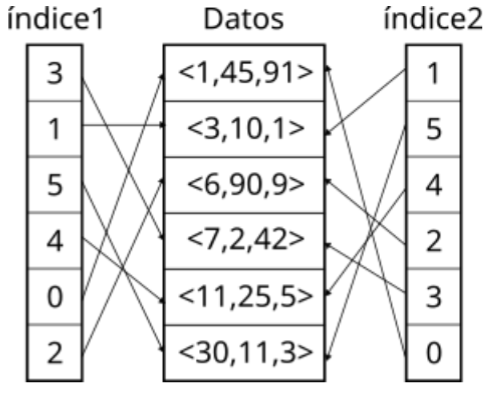
\includegraphics[width=7cm]{./indices.png}
\end{figure}

En la figura, si recorremos los datos en el orden en el que están guardados, obtenemos:
\[[<1,45,91>,<3,10,1>,<6,90,9>,<7,2,42>,<11,25,5>,<30,11,3>]\]
Si lo recorremos usando el índice 1 (que apunta a los elementos en función de la segunda componente) obtenemos:
\[[<7,2,42>,<3,10,1>,<30,11,3>,<11,25,5>,<1,45,91>,<6,90,9>]\]

\begin{itemize}
	\item Escriba la estructura propuesta
	\item Escriba el InvRep y la func Abs, en castellano y en lógica para el TAD Conjunto(Tupla($\ent,\ent,\ent$))
	\item Escriba el algoritmo de BuscarPor que busca por alguna componente
	\item Escriba los algoritmos de agregar y sacar
\end{itemize}

TuplaEnt es \tupla{\Int,\Int,\Int}
\begin{module}{Conjunto}{TuplaEnt}{Conjunto}{\tupla{\ent,\ent,\ent}}
	\var{conj}{\Array{TuplaEnt}}
	\var{indices}{\tupla{\Array{\Int},\Array{\Int},\Array{\Int}}}

	\pred{sinRepetidos}{a: \Array{T}}{
		\paraTodo{i,j}{\Int}{0 \leq i < j < length(a) \thenLuego a[i] \neq a[j]}
	}

	\pred{indiceValido}{a: \Array{TuplaEnt}, indice: \Array{\Int}, comp: \Int}{
		length(a) = length(indice) \land \\
		\paraTodo{i}{\Int}{i \in indice \iff 0 \leq i < length(a)} \yLuego \\
		\paraTodo{i}{\Int}{0 \leq i < length(indice) - 1 \thenLuego a[indice[i]]_{comp} \leq a[indice[i + 1]]_{comp}}
	}

	\pred{InvRep}{c: \moduletype}{
		sinRepetidos(c.conj) \land \\
		\paraTodo{comp}{\Int}{0 \leq comp < length(c.indices) \thenLuego indiceValido(c.conj, indices[comp], comp)}
	}

	\pred{predAbs}{c1: \moduletype, c2: \tadtype}{
		\paraTodo{e}{\ent}{e \in c2.elems \iff \existe{i}{\Int}{0 \leq i < length(c1.conj) \yLuego c1.conj[i] = e}}
	}

	\pagebreak

	\begin{proc}{BuscarPor}{\In c: \moduletype, \In comp: \Int, \In e: \Int}{TuplaEnt}
		\begin{lstlisting}[numbers=none,frame=none]
		var der: int;
		var izq: int;
		var med: int;
		izq := 0;
		der := length(c.conj) - 1;

		if c.conj[indices[comp][der]][comp] == e
			return c.conj[indices[comp][der]];
		endif

		while izq + 1 < der do
			med := floor((izq + der) / 2);
			if c.conj[indices[comp][med]][comp] <= e
				izq = med;
			else
				der = med;
			endif
		endwhile

		if c.conj[indices[comp][izq]][comp] == e
			return c.conj[indices[comp][izq]];
		endif

		return null;
		\end{lstlisting}
	\end{proc}

	\begin{proc}{agregar}{\Inout c: \moduletype, \In t: TuplaEnt}{}
		\begin{lstlisting}[numbers=none,frame=none]
		var i: int;
		var aux: Array < TuplaEnt >;
		var comp: int;
		i := 0;
		comp := 0;
		aux := new Array < TuplaEnt >(length(c.conj) + 1);

		while i < length(c.conj) do
			aux[i] := c.conj[i];
			i := i + 1;
		endwhile

		aux[length(c.conj)] := t;

		c.conj = aux;

		while comp < length(c.indices) do
			agregarEnIndice(c, comp, t);
			comp := comp + 1;
		endwhile
		\end{lstlisting}
	\end{proc}

	\pagebreak

	\begin{proc}{agregarEnIndice}{\Inout c: \moduletype, \In comp: \Int, \In t: TuplaEnt}{}
		\begin{lstlisting}[numbers=none,frame=none]
		var aux: Array < int >;
		var i: int;
		var insertado: bool;

		aux := new Array < int >(length(c.indices[comp]) + 1);
		i := 0;
		insertado := false;

		while i < length(c.indices[comp]) do
			if insertado
				aux[i+1] := c.indices[comp][i];
				i := i + 1;
			else if c.conj[c.indices[comp][i]][comp] > t[comp]
				aux[i] := t;
				insertado := true
			else
				aux[i] := c.indices[comp][i];
				i := i + 1;
			endif
		endwhile

		c.indices[comp] = aux;
		\end{lstlisting}
	\end{proc}

	\begin{proc}{sacar}{\Inout c: \moduletype, \In t: TuplaEnt}{}
		\begin{lstlisting}[numbers=none,frame=none]
		var i: int;
		var comp: int;
		var aux: Array < TuplasEnt >;
		var borrado: bool;
		i := 0;
		comp := 0;
		aux := new Array < TuplasEnt >(length(c.conj) - 1)
		borrado := false;

		while comp < length(c.indices) do
			sacarEnIndice(c, comp, t);
			comp := comp + 1;
		endwhile

		while i < length(c.conj) do
			if borrado
				aux[i - 1] := c.conj[i];
			else if c.conj[i] != t
				aux[i] := c.conj[i];
			endif

			i := i + 1;
		endwhile

		c.conj = aux;
		\end{lstlisting}
	\end{proc}

	\pagebreak

	\begin{proc}{sacarEnIndice}{\Inout c: \moduletype, \In comp: \Int, \In t: TuplaEnt}{}
		\begin{lstlisting}[numbers=none,frame=none]
		var i: int;
		var borrado: bool;
		var aux: Array < int >;
		i := 0;
		borrado := false;
		aux := new Array < int >(length(c.indices[comp]) - 1);

		while i < length(c.indices[comp]) do
			if borrado
				aux[i - 1] := c.indices[comp][i];
			else if c.conj[c.indices[comp][i]] == t
				borrado := true;
			else
				aux[i] := c.indices[comp][i];
			endif

			i := i + 1;
		endwhile

		c.indices[comp] = aux;
		\end{lstlisting}
	\end{proc}
\end{module}

\subsection{Ejercicio 5}
Una forma eficiente de implementar el TAD Cola en su versión acotada, es mediante un \textit{buffer circular}. Esta estructura está formada por un array del tamaño maximo de la cola (\textit{n}) y dos índices (\textit{inicio} y \textit{fin}), para indicar adonde empieza y adonde termina la cola. El chiste de esta estructura es que, al llegar al final del arreglo, si los elementos del principio ya fueron consumidos, se puede reusar dichas posiciones.

\begin{figure}[h!]
	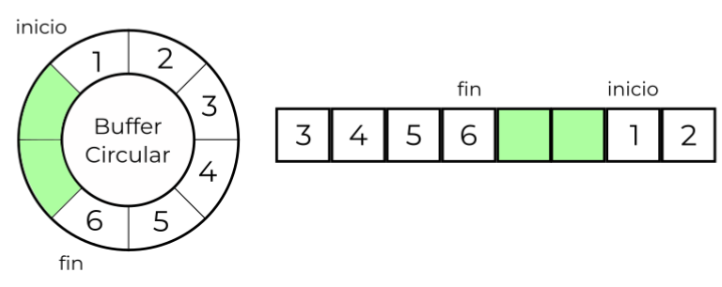
\includegraphics[width=10cm]{./buffer_circular.png}
\end{figure}

\begin{itemize}
	\item Elija una estructura de representación
	\item Escriba el invrep y la func abs
	\item Escriba los algoritmos de las operaciones encolar y desencolar
	\item ¿Por qué tiene sentido utilizar un buffer circular para una cola y no para una pila?
\end{itemize}

\pagebreak

\begin{module}{ColaBufferCirc}{T}{ColaAcotada}{T}
	\var{elems}{\Array{T}}
	\var{inicio}{\Int}
	\var{fin}{\Int}

	\pred{InvRep}{c: \moduletype}{
		\hacer
	}

	\pred{predAbs}{c1: \moduletype, c2: \tadtype}{
		\hacer
	}

	\begin{proc}{encolar}{\Inout c: \moduletype, \In e: T}{}
		\begin{lstlisting}[numbers=none,frame=none]
		if c.fin == -1
			c.fin := c.inicio;
		else
			c.fin := (c.fin + 1) % length(c.elems);
		endif

		c.elems[c.fin] := e;
		cant := cant + 1;
		\end{lstlisting}
	\end{proc}

	\begin{proc}{desencolar}{\Inout c: \moduletype}{}
		\begin{lstlisting}[numbers=none,frame=none]
		c.inicio := (c.inicio + 1) % length(c.elems)
		cant := cant - 1;
		\end{lstlisting}
	\end{proc}

\end{module}

\subsection{Ejercicio 6}
\hacer

\end{document}
